
%(BEGIN_QUESTION)
% Copyright 2011, Tony R. Kuphaldt, released under the Creative Commons Attribution License (v 1.0)
% This means you may do almost anything with this work of mine, so long as you give me proper credit

Tegn inn alle nødvendige ledninger og rør for å gjøre dette til et fungerende reguleringssystem, og legg til eventuelle komponenter som mangler:

$$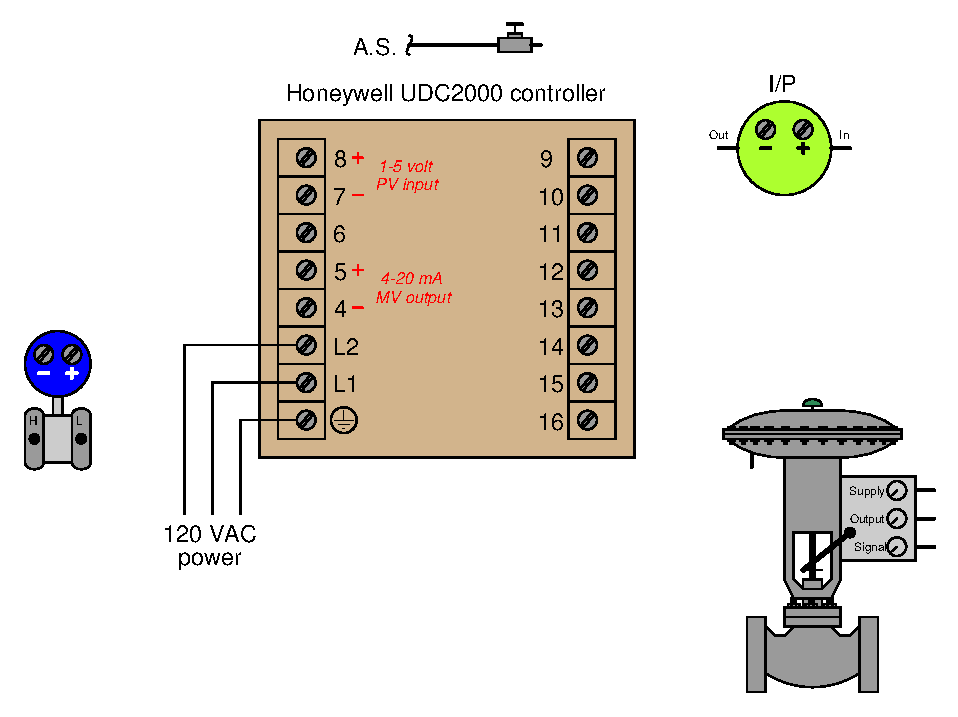
\includegraphics[width=15.5cm]{i00663x01.eps}$$

\underbar{file i00663no}
%(END_QUESTION)





%(BEGIN_ANSWER)

Gi halv uttelling hvis bare inngangskablingen er riktig, eller hvis bare utgangskablingen (og rørføringen) er riktig:

$$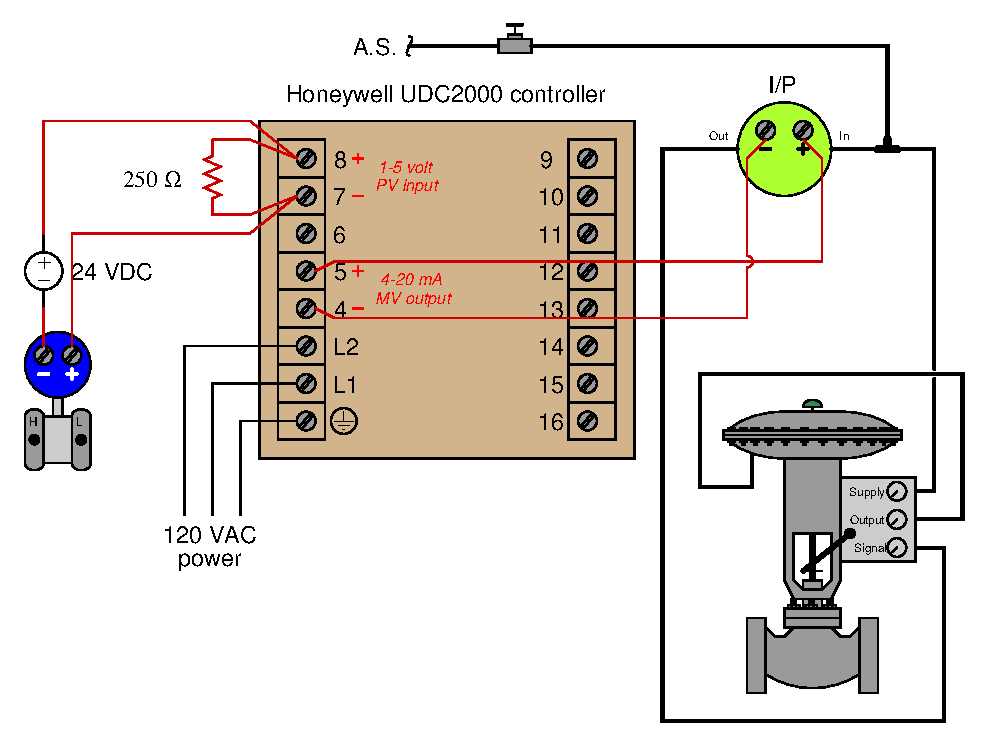
\includegraphics[width=15.5cm]{i00663x02.eps}$$

Trekk 2 poeng hvis ingen motstandsverdi er oppgitt (250 ohm).

%(END_ANSWER)





%(BEGIN_NOTES)

{\bf Denne oppgaven er ment for eksamen, ikke arbeidsark.}

%(END_NOTES)
